\section{Register and State Abstraction}
\label{sec:state_abstractions}
\begin{table*}
  \begin{threeparttable}
  \captionof{table}{State Semantics Example Function, $g$: Definition and Implementations}
	\label{tbl:StateExDefImpl}
	\setlength\tabcolsep{1.5pt}
  \begin{tabular}{|c|c|c|c|c|}
  \hline 
  \textbf{Formal Definition} & \textbf{Functional Drawing} & \textbf{C++ Impl.}\tnote{†}~\tnote{‡} & \textbf{VHDL Impl.}\tnote{‡} & \textbf{DFiant Impl.} \\ 
  \hline
	\begin{minipage}[b][3.2cm][c]{0.21\linewidth}
    {\fontsize{8}{8}\selectfont
		\begin{equation}
			\nonumber
      \begin{split}
			&g:(i_{n})_{n\in \mathbb{N}}\rightarrow (a_n,b_n,c_n)_{n\in \mathbb{N}}\\  
      &\triangleq\left\{
      \begin{aligned}
      a_k &= i_k+5 & k\geq 0\\ 
      b_k &= i_k+i_{k-1} & k>0 \\   
      b_k &= i_k+0  & k=0 \\
      c_k &= i_k+c_{k-1} & k>0  \\ 
      c_k &= i_k+0 & k=0
      \end{aligned} 
      \right.
      \end{split}
		\end{equation}
    }
	\end{minipage}
  &
	\begin{minipage}[b][3.2cm][c]{0.18\linewidth}
    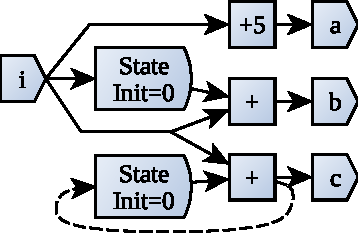
\includegraphics[width=\linewidth]{graphics/gFuncDraw.pdf}
  \end{minipage}%
  &
	\begin{minipage}[b]{0.14\linewidth}
		\begin{minted}[autogobble,tabsize=2,fontsize=\fontsize{8}{8}\selectfont]{c}
      void g(int i,
             &a,&b,&c){
        static int î=0;
        static int C=0;
        
        a = i + 5;
        b = i + î;
        î = i;
        c = i + C;
        C = c;
      }
		\end{minted}
	\end{minipage}
	&
	\begin{minipage}[b]{0.21\linewidth}
		\begin{minted}[autogobble,tabsize=2,fontsize=\fontsize{8}{8}\selectfont]{vhdl}
      g : process(clk)
        variable î : integer:=0;
      begin
        if rising_edge(clk)
        begin
          a <= i + 5;
          b <= i + î;
          î := i;
          c <= i + c;
        end; 
      end process;
			\end{minted}
	\end{minipage}
	&
	\begin{minipage}[b]{0.23\linewidth}
		\begin{minted}[autogobble,tabsize=2,fontsize=\fontsize{8}{8}\selectfont]{scala}
      def g(i : DFSInt[32]) = 
      {
        
        
        
        val a = i + 5
        val b = i + i.init(0).prev
        val c = DFSInt[32]
        c := i + c //prev optional
        (a,b,c.prev) //tuple of 3
      }
		\end{minted}
	\end{minipage}
  \\
  \hline
  \end{tabular}
  \begin{tablenotes}
    \item [†] Some type annotations were removed for brevity.
    \item [‡] \textbf{î} and \textbf{C} represent previous state values of \textbf{i} and \textbf{c}, respectively.
  \end{tablenotes}
  \end{threeparttable}
\end{table*}%

In the previous section we compared implementations of a pure (stateless) function, $f$. Typical designs, however, possess a state that is implemented via clocked registers. Registers have other functional roles, such as pipelining a data path, deriving timed signals from an input clock, and synchronizing an input signal. We believe that by avoiding explicit register use, we can design without, or very little, clock dependency. 

In this section we classify various register use-cases, and present their DFiant functional counterpart. The classifications are divided into three main categories: \textit{synchronous technology backend}, \textit{synchronous technology interface}, and \textit{state}. For the state classification, we also explore an impure function, $g$, and compare its implementation in VHDL, C++, and DFiant (see Table~\ref{tbl:StateExDefImpl}).

%Clocked registers have various functional roles, yet all appear the same in modern HDL designs. 
%The main reason is that devices have very small number of IO ports, measurable in the hundreds, while modern designs process trillions of bps. Designs are This, of course, forces existance of state, since pure functions must receive all inputs  . Therefore, it is impossible to avoid state in a full (\textit{top}) system hardware description. 
%When HLS abstract away the clock, it is left to the code analysis to classify what variable hold state.

\subsection{Synchronous Technology Backend}
Registers are often forced upon the design due to a synchronous technology choice. Since they are unrelated to the functional requirement, DFiant has no constructs to express them, and relies on its compiler to implement them properly based on the functional requirements and design constraints.
We differentiate between the following backend register uses:
\subsubsection{Pipelining}
DFiant auto-pipelines the design by inserting registers to split long combinational paths. The amount of pipelining is determined by designer-specified constraints, such as the maximum path cycle latency, or the maximum propagation delay between registers.
\subsubsection{Synchronizers}
Sampling clock domain crossing (CDC) or asynchronous signals is exposed to metastability. Synchronizers, often composed of registers, are used to mitigate its effect and bring the design to the proper reliability. Since we aspire for a clockless design frontend, we want the synchronizers to be implicit. Currently, DFiant only supports a single clock backend, and does not require synchronizers. Further research may explore other backend options.

\subsection{Synchronous Technology Interface}
Functional design requirements are often accompanied by synchronous input/output (IO) timing constraints such as clocked protocol interfaces or real-time restrictions. However, these constraints only effect the interface, and are unrelated to the design core. To maximize design portability, we apply legacy constructs solely in the periphery, while keeping the design core coded in dataflow. DFiant exposes a frontend bridge across legacy RTL constructs and its dataflow types. We differentiate between the following synchronous signaling:
\subsubsection{External IO and Blackbox Interfaces}
External IOs that are exposed to the top design hierarchy, or blackboxes that are exposed to the internal design core, may impose synchronous protocols (e.g., data is valid one clock cycle after address is set). DFiant supports legacy RTL constructs to synchronously interface external IOs and instantiate blackboxes. 
%We implemented a preliminary interface between DFiant and Chisel, allowing us to tap into Chisel's hardware generation and cycle accurate simulations.
\subsubsection{Timers}
Timers are design constructs for outputting real-time signals, or creating derivations of timed signal inputs. For example, a target device is fed by a 100MHz clock and we want to output a UART stream at 10Mbps or toggle a led at 1Hz. Instead of directly applying registers or clock generation components, we can create functional representation of their timed use-cases. Currently, DFiant supports timers with legacy RTL constructs. This work may be expanded to include functional timers.

\subsection{State}
State occurs when we require access to (previous) values which are no longer available on a function's inputs (e.g., cumulative sum or a state-machine's state). Table~\ref{tbl:StateExDefImpl} introduces a state function, $g$, and its implementation in C++, VHDL, and DFiant. The C++ implementation uses the \code{static} keyword to create variables that maintain the history of \code{i} and \code{c}. Because a static variable saves its value for every call of \code{g}, the C++ implementation cannot be used in the same design more than once. The VHDL implementation invokes registers (behaviorally) to save the state. Unfortunately, registers not only save the state, but also enforce specific cycle latencies. Furthermore, both C++ and VHDL declare additional variables and place extra assignments just to save the state. DFiant overcomes all these issues and in a less cumbersome way.

The DFiant state abstraction is achievable via the \code{.prev} construct, to summon the previous dataflow variable value, and also the construct \code{.init(value)}, to create an initialized dataflow variable. The \code{:=} assignment operation is available for a mutable dataflow variable such as \code{c} (see Section~\ref{sec:mutability}). The creation of \code{c} carries within it an implicit assignment \code{c := c.init(0).prev}, which makes the next assignment of \code{c}, \code{c := i + c}, equivalent to \code{c := i + c.init(0).prev}. This is possible due to the following semantics: \textit{previous values change at the end of the DFiant code} (similarly to signal update semantics in VHDL processes). One advantage is that the code resembles its RTL counterparts, but less verbose. Another advantage is that any type of state component, like the Muller C-element\cite{muller1957theory}, can be applied with DFiant as a frontend (note that the functional drawing in Table~\ref{tbl:StateExDefImpl} has no register drawn).

%entire design or process loop semantics. DFiant variables are implicitly static.
%Functionally a register is a memory with a single write port and unlimited

We differentiate between two kinds of state: \textit{derived state}, and \textit{regular state}. Addressable memory pools also hold state, but we currently classify them as blackboxes. %Future work may provide dedicated functional abstractions for such components as well.

\subsubsection{Derived State} 
A derived state is a state whose current output value is \textit{independent} of its previous value. For example, calculating output \code{b} of function \code{g} requires summoning previous value of \code{i}. 

\subsubsection{Regular State} 
A regular state is a state whose current output value is \textit{dependent} of its previous state value. For example, the cumulative sum output, \code{c}, of function \code{g} is dependent on the old sum value. 

The two types of state differ heavily in performance improvement when the design is pipelined. A path from \code{i} to \code{b} can produce a token for every clock tick, and if we pipeline the addition operation to increase the maximum frequency, the maximum throughput will increase as well. Contrarily, a path from \code{i} to \code{c} also depends on the previous value of \code{c}, and if we pipeline the addition operation of that path, the extra latency may even decrease the throughput (multi-cycle path). Furthermore, \code{i} is forked into several paths, and  abides by the slowest path throughput. 

Regular state causes bottlenecks in many systems. For instance, a processor's program counter (PC) register manifests as a regular state. The processor pipeline can only be improved thanks to a speculative mechanism that predicts the next PC value to prefetch instructions (e.g., PC+4 for a branch-not-taken prediction). In case of a miss-prediction, other mechanisms take place. Further research may expand DFiant's abstractions, and solve such problems functionally.

%\subsubsection{Speculated State} 
%A speculated state is a regular state that can generate a new speculative value when the actual next value is unavailable.

%In some cases a regular state limits the throughput too much. For example, a program counter (PC) register for a microprocessor pipeline. If we state dependent on the PC as a regular state, it won't be possible for the pipeline to handle more than one instruction at a time. A known solution for this is to speculate on the next value of PC (good guess is branch not taken). If we guessed wrong the pipeline should ignore the prefetched instructions and restart from where the branch occurred. This allows us to generate new speculative tokens of PC, without waiting for the pipeline to supply the vi

%There is no actual dataflow feedback. 
